\documentclass[tikz,border=5pt]{standalone}
\usepackage{fontspec}
\setmainfont{Times New Roman}
\usepackage{unicode-math}
\setmathfont{Cambria Math}
\usetikzlibrary{shapes.geometric,shapes.misc,positioning,fit,backgrounds,arrows.meta,calc}

\begin{document}
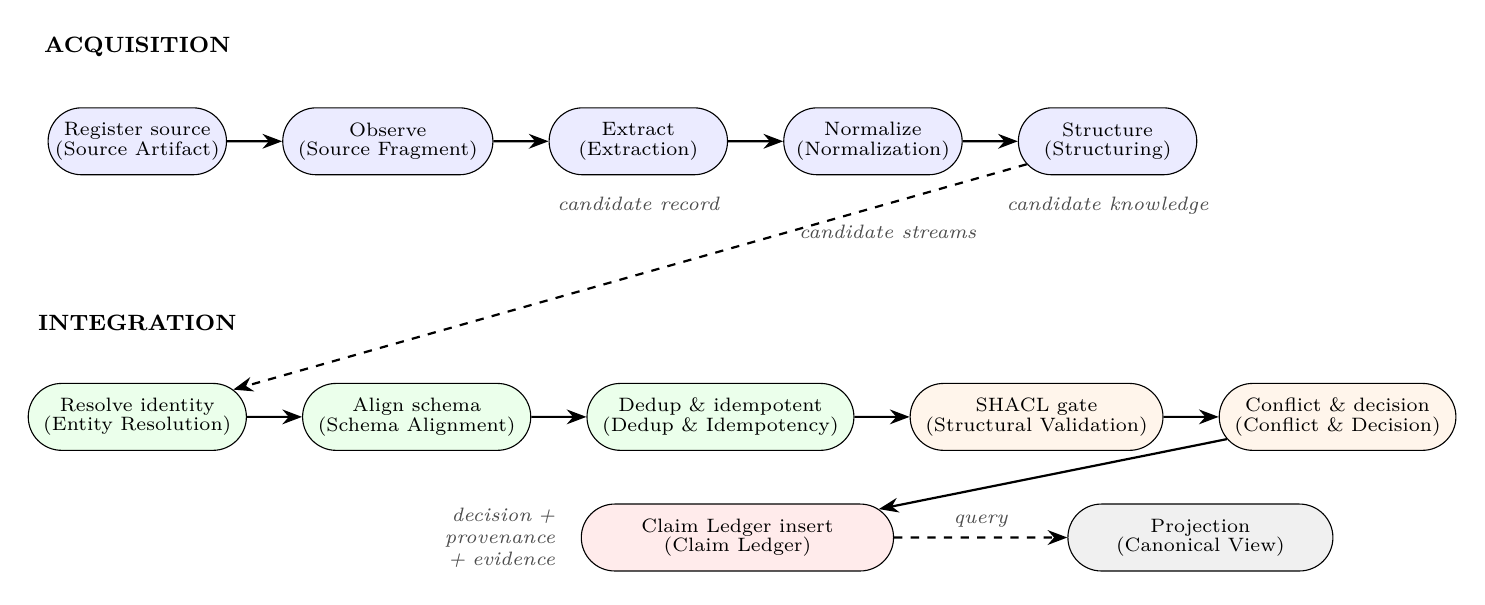
\begin{tikzpicture}[
    node distance=1.0cm and 0.7cm,
    stage/.style={rounded rectangle, draw, minimum width=2.5cm, minimum height=0.85cm, align=center, font=\scriptsize},
    arrow/.style={-{Stealth[length=2.5mm]}, thick},
    label/.style={font=\scriptsize\itshape, text=gray!60!black},
    phase/.style={font=\footnotesize\bfseries},
]

% ================== Acquisition phase ==================
\node[phase] (acqTitle) at (0, 4.4) {ACQUISITION};
\node[stage, fill=blue!8] (s1) at (0, 3.2) {Register source\\[-1pt]\scriptsize(Source Artifact)};
\node[stage, fill=blue!8, right=of s1] (s2) {Observe\\[-1pt]\scriptsize(Source Fragment)};
\node[stage, fill=blue!8, right=of s2] (s3) {Extract\\[-1pt]\scriptsize(Extraction)};
\node[stage, fill=blue!8, right=of s3] (s4) {Normalize\\[-1pt]\scriptsize(Normalization)};
\node[stage, fill=blue!8, right=of s4] (s5) {Structure\\[-1pt]\scriptsize(Structuring)};

\draw[arrow] (s1) -- (s2);
\draw[arrow] (s2) -- (s3);
\draw[arrow] (s3) -- (s4);
\draw[arrow] (s4) -- (s5);

\node[label, below=0.15cm of s3] {candidate record};
\node[label, below=0.15cm of s5] {candidate knowledge};

% ================== Integration phase ==================
\node[phase] (intTitle) at (0, 0.9) {INTEGRATION};
\node[stage, fill=green!8] (i1) at (0, -0.3) {Resolve identity\\[-1pt]\scriptsize(Entity Resolution)};
\node[stage, fill=green!8, right=of i1] (i2) {Align schema\\[-1pt]\scriptsize(Schema Alignment)};
\node[stage, fill=green!8, right=of i2] (i3) {Dedup \& idempotent\\[-1pt]\scriptsize(Dedup \& Idempotency)};
\node[stage, fill=orange!8, right=of i3] (i4) {SHACL gate\\[-1pt]\scriptsize(Structural Validation)};
\node[stage, fill=orange!8, right=of i4] (i5) {Conflict \& decision\\[-1pt]\scriptsize(Conflict \& Decision)};

\draw[arrow] (i1) -- (i2);
\draw[arrow] (i2) -- (i3);
\draw[arrow] (i3) -- (i4);
\draw[arrow] (i4) -- (i5);

% ================== Ledger ==================
\node[stage, fill=red!8, minimum width=4.2cm, below=1.1cm of $(i1)!0.5!(i5)$] (ledger) {Claim Ledger insert\\[-1pt]\scriptsize(Claim Ledger)};
\draw[arrow] (i5) -- (ledger);
\node[label, left=0.2cm of ledger, align=right, text width=2.6cm] {decision +\\provenance + evidence};

% Bridge between phases
\draw[arrow, dashed] (s5) -- node[label, right, pos=0.3] {candidate streams} (i1);

% ================== Projection ==================
\node[stage, fill=gray!12, minimum width=3.6cm, right=2.2cm of ledger] (proj) {Projection\\[-1pt]\scriptsize(Canonical View)};
\draw[arrow, dashed] (ledger) -- node[label, above] {query} (proj);

\end{tikzpicture}
\end{document}
